%%%%%%%%%%%%%%%%%%%%%%%%%%%%%%%%%%%%%%%%%%
% Master Thesis 
% Polina Polunina
% October 2022 
%
% License:
% CC-BY-SA 4.0 -- Creative Commons Attribution-ShareAlike 4.0 International
% https://creativecommons.org/licenses/by-sa/4.0/legalcode
%%%%%%%%%%%%%%%%%%%%%%%%%%%%%%%%%%%%%%%%%%
\section{Results} \label{sec:results}
In the following sections, the results of downstream data analysis will be shown. In \cref{sec:results:mock}, results and analysis on a mock synthetic dataset will be presented, followed by \cref{sec:results:real}, where results obtained by running workflows on real datasets will be shown and described.

    \subsection{Mock dataset results} \label{sec:results:mock}
    Mock dataset has been synthetically generated by a working group and is available on GitHub. Synthetic dataset of overall 100 samples was created by obtaining genomes from the Pango designation list using three real variants (BA.1, BA.2, Delta), one synthetic background variant (BG), and recombinant genomes (Omicron-Delta). Synthetic amplicons were created using ARTIC v4.1 primers. Short 150 bp and long 250 bp reads were used while generating. Briefly, the mock dataset can be described by belonging samples to groups of different classes such as: i) Single lineage, Two lineages, Three lineages; ii) High coverage, Low coverage; iii) Long reads, Short reads. Details on the number of mock samples of each group are in \cref{tab:methods:mock}.
    
    From 100 mock samples: 22 contain single lineage, 42 - two distant lineages (BA.1 and Delta), 6 - two close lineages (BA.1 and BA.2), 14 samples - 2 known and one unknown lineage (synthetically generated), 8 samples - known lineages, and 8 samples - 3 known and one unknown lineages. On the other hand, the mock dataset contains 50 samples of low coverage and 50 samples of low coverage. The mock samples consist of 24 long reads (250 base pairs) and 76 short reads (150 base pairs).
    
    For the evaluation of workflows developed for ampliconic data, the workflow’s Freyja-based and COJAC-based branches as well as the standalone Lineagespot workflow were run on a mock dataset.
    
        \subsubsection{Benchmarking Galaxy and Lineagespot workflow results}
        Galaxy workflows results were compared with Lineagespot results using the same synthetic mock dataset. As expected, Galaxy workflow results in both branches differ from Lineagespot results. That is because different approaches (sub-workflows) are used for data preprocessing steps which were described in \autoref{sec:methods:evaluation:mock:compare-ls} of \cref{sec:methods}. In evaluating workflows on the mock dataset, two groups of samples were selected: one with a single lineage and one with two lineages.
            \paragraph{Single lineage group of samples}
            The Single lineage group consists of 22 samples. Four characteristics were used for a single lineage group. The goal was to discover in which samples were detected: i) expected lineage; ii) expected lineage plus unexpected lineages; iii) unexpected lineage; iv) nothing. Each of these characteristics is represented by a combined bar plot that shows how many samples meet that characteristic.
                \subparagraph{Bar plot}
                From \cref{fig:results:mock:bar-singlin} it is obvious that all three tools are effective in detecting expected lineage. Nonetheless, in the detection of only expected lineage and nothing more, Lineagespot performed the best, compared to COJAC and Freyja. Freyja is effective at detecting expected lineage; however, it always detected some unexpected lineages. COJAC's results are close to Freyja's results, but COJAC was able to detect 2 samples with the expected lineage. Another interesting observation is that in 4 samples, COJAC is rather to detect nothing than expected lineage. 
                \begin{figure}[ht!]
                	\centering
                    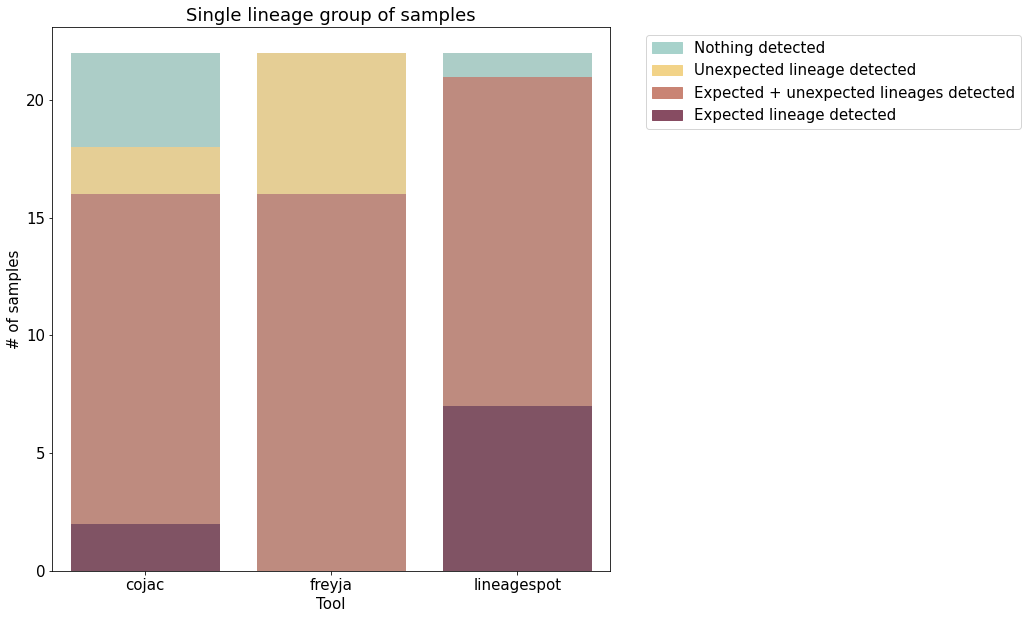
\includegraphics[width=0.8\textwidth]{figures/results/mock/singlin-num-bars.png}
                    \captionof{figure}{Bar plot describing the number of mock samples of single lineage group that meet one of four characteristics: i) expected lineage detected; ii) expected lineage plus unexpected lineages detected; iii) unexpected lineage detected; iv) nothing detected}
                    \label{fig:results:mock:bar-singlin}
                \end{figure}
                \Cref{fig:results:mock:bar-singlin} shows that Freyja is an effective tool for detecting expected lineage, even though Freyja always detects other lineages. When it is expected the sample to contain only one lineage but nothing more, Freyja is not that effective. Moreover, in 6 samples for Freyja and in 2 samples for COJAC (out of 22), there were detected unexpected, i.e. incorrect, lineages. On the other hand, Lineagespot is effective in the case of detecting only expected lineages, probably because it has the additional step in its pipeline when the most probable lineages are assigned for the sample. This extra step is made based on several indicators. So Lineagespot detected only expected lineage in 7 samples out of 22 samples from a single lineage group. As for COJAC, it performed quite well and was able to detect only one lineage that was expected in 2 out of 22 samples, however, for 4 samples with expected lineage, COJAC detected nothing.
                
                \subparagraph{Venn Upset}
                In order to better understand the interrelationships between different results (Freyja, COJAC, Lineagespot), a Venn Upset diagram was generated. Using this method, I analyzed intersections between sets of results and determined which samples were correctly detected by which tool (in terms of the lineages expected) and how similar the results were between tools.

                Venn Upset diagram below (\cref{fig:results:mock:venn-singlin}) was constructed based on 22 samples in which there was a single lineage expected. Each column corresponds to a set of obtained results from certain tools (COJAC, Lineagespot, Freyja), and bar charts on top show the size of the set of tool’s results. The first row in the figure is completely empty, while 1 sample is expected to be detected but was not. This sample75 is expected to contain only unknown synthetic lineage. 
                
                The second row corresponds to 5 samples with the expected single lineage only detected by Lineagespot but not by COJAC and Freyja. Finally, the last third row represents 16 samples with the expected single lineage detected by all tools. Freyja and COJAC detected the expected lineage only in 16 samples which are confirmed in the bar plot above (\cref{fig:results:mock:bar-singlin}).
                \begin{figure}[ht!]
                	\centering
                    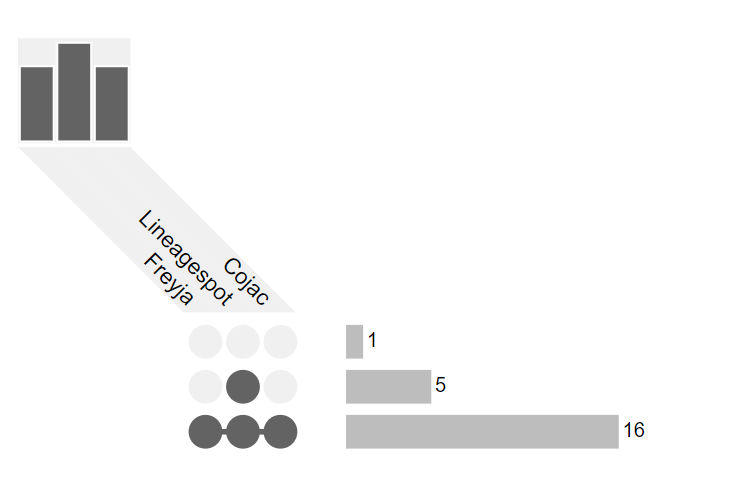
\includegraphics[width=0.7\textwidth]{figures/results/mock/venn-singlin.png}
                    \captionof{figure}{Venn Upset diagram constructed based on 22 samples in which there was single lineage expected.}
                    \label{fig:results:mock:venn-singlin}
                \end{figure}

                \subparagraph{Distribution: proportion of expected lineage detected by tool}
                Moreover, using Python with the Seaborn library, a distribution of the proportion of lineage detected by Freyja and COJAC among samples in the Single lineage group was plotted (\cref{fig:results:mock:dist-singlin}) by only considering samples where expected lineage was detected. The comparison was limited to Freyja and COJAC. In Lineagespot, I do not have a clean proportion distribution between lineages, so I do not consider it here. One of the reasons for excluding Lineagespot from this distribution analysis: besides BA.1, BA.2, Delta, no information was provided about other lineages that have been detected in Lineagespot, and the sum of proportions of these three does not equal 1. 
                \begin{figure}[ht!]
                	\centering
                    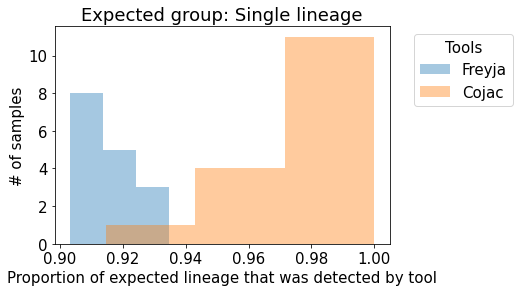
\includegraphics[width=0.7\textwidth]{figures/results/mock/dist-singlin-fr-co.png}
                    \captionof{figure}{Distplot that represents the distribution of lineage proportion detected by Freyja and COJAC among samples of the Single lineage group, considering only samples in which expected lineage was detected.}
                    \label{fig:results:mock:dist-singlin}
                \end{figure}
                Looking at \cref{fig:results:mock:dist-singlin}, I conclude that for single lineage detection, the results of lineage proportion from COJAC and Freyja are from 0.9 to 1. However, some differences between Freyja and COJAC results are observed. Freyja showed a lower proportion of expected lineage, while for COJAC the proportion tends to 1 which is expected. Thus, we can guess that COJAC results for the single lineage group are closer to what was expected.
                
                \subparagraph{Parallel coordinates}
                For comparing Freyja and COJAC results with each other and with expected results, parallel coordinates plots were created using Python and Plotly graphing libraries. Samples are plotted as parallel coordinates across different measures using this visualization technique. Samples are represented as connected points along each vertical axis, and each measure corresponds to a vertical axis. 

                Three plots, focused on the group of samples marked as "single lineage", were generated for Delta (\cref{fig:results:mock:pc-singlin-delta}), BA.1 (\cref{fig:results:mock:pc-singlin-ba1}), and BA.2 (\cref{fig:results:mock:pc-singlin-ba2}) lineages. Graphs represent different lineages (one lineage per graph). Within the graph, the left axis represents the expected proportion, the middle axis represents proportion of Delta lineage detected by COJAC, while right axis represents the proportion of Delta lineage detected by Freyja.
                
                \begin{figure}[H]
                    \begin{subfigure}{\linewidth}
                	\centering
                    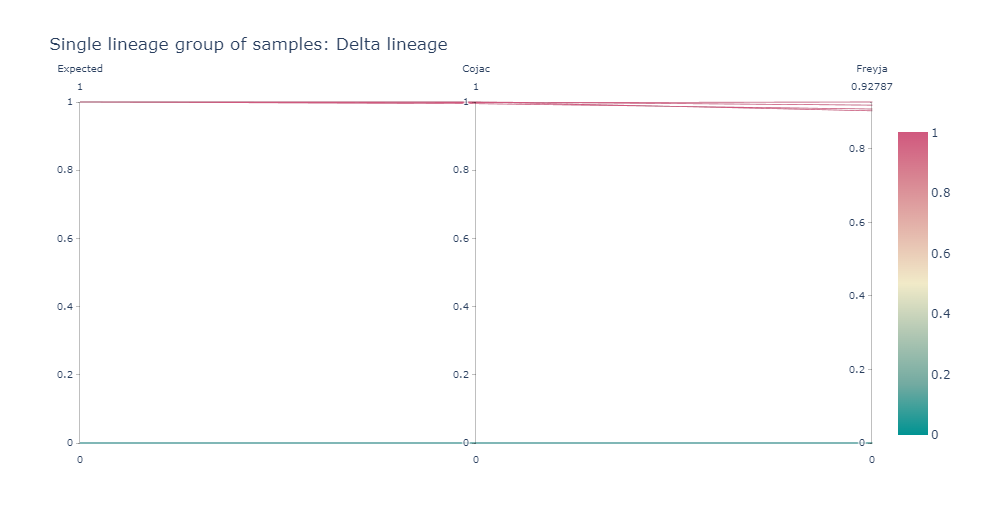
\includegraphics[width=0.75\textwidth]{figures/results/mock/pc-singlin-delta.png}
                    \captionof{figure}{Delta}
                    \label{fig:results:mock:pc-singlin-delta}
                    \end{subfigure}\par\medskip
                    \begin{subfigure}{\linewidth}
                	\centering
                    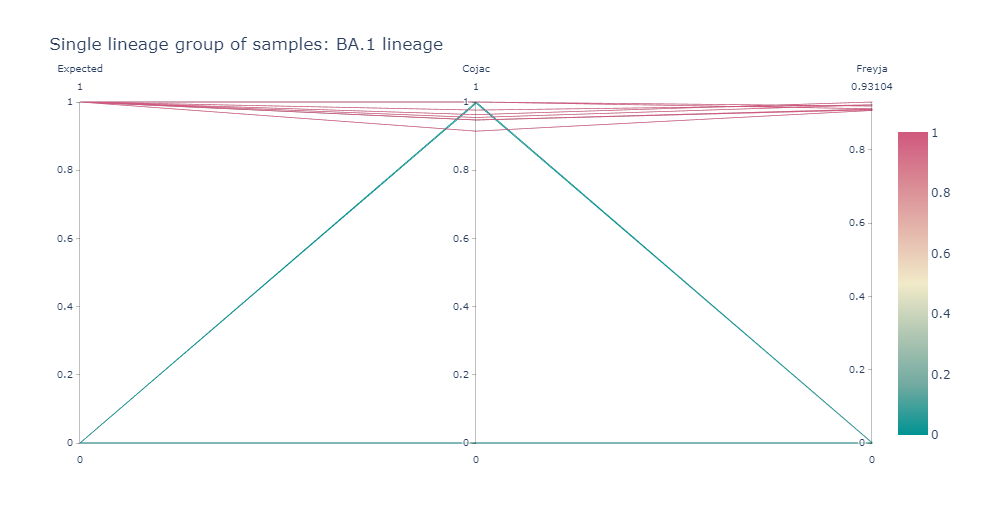
\includegraphics[width=0.75\textwidth]{figures/results/mock/pc-singlin-ba1.png}
                    \captionof{figure}{BA.1}
                    \label{fig:results:mock:pc-singlin-ba1}
                    \end{subfigure}\par\medskip
                    \begin{subfigure}{\linewidth}
                	\centering
                    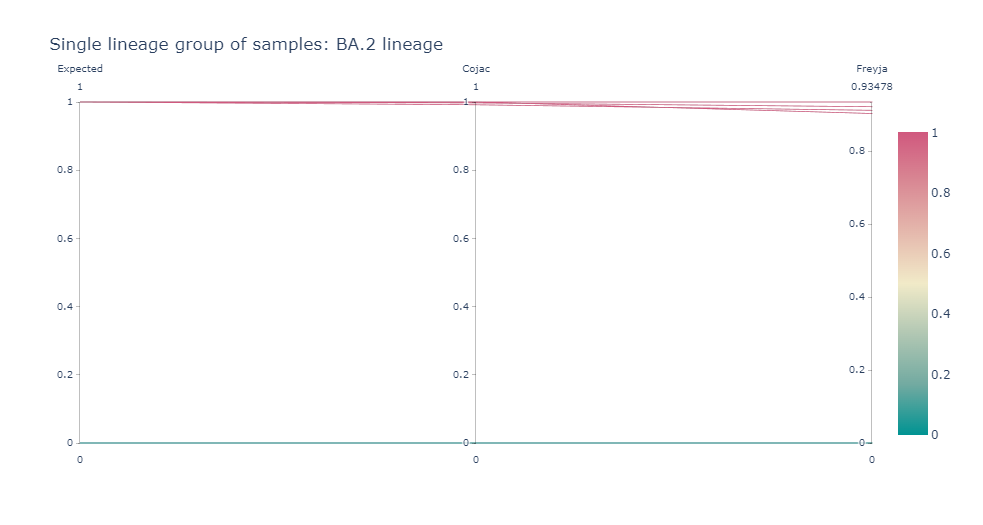
\includegraphics[width=0.75\textwidth]{figures/results/mock/pc-singlin-ba2.png}
                    \captionof{figure}{BA.2}
                    \label{fig:results:mock:pc-singlin-ba2}
                    \end{subfigure}\par\medskip
                    \captionof{figure}{Parallel coordinates plot for a single lineage group of samples that compare the lineage proportions detected by Freyja and COJAC with each other as well as with expected proportion. The left axis represents the expected proportion of the lineage, the middle axis represents the proportion of the lineage detected by COJAC, while the right axis represents the proportion of the lineage detected by Freyja.}
                \end{figure}
                
                From \cref{fig:results:mock:pc-singlin-delta} and \cref{fig:results:mock:pc-singlin-ba2}, it is observed that for single lineage group of samples, for detecting Delta and BA.2, COJAC performs well, the value of proportion is very close to expected 1, while Freyja performs slightly below expected. However, both results are close to expected for all samples of this group (Single lineage group).

                Quite a bit different results are shown in \cref{fig:results:mock:pc-singlin-ba1}, for BA.1 lineage. More specifically, Cojac’s results for a few samples are closer to Freyja’s results, with a value of 0.9, whereas a value of 1 is expected. In another curious case, for sample83 and sample52 BA.1 lineage was not expected. Freyja did not detect this lineage. COJAC, in turn, detected 0.9962962963 proportion of BA.1 lineage for sample83, and 1 for sample52, which is high. The explanation for this is that in the mock dataset, these two samples contain only recombinant (BA.1+BA.2+Delta). It is also possible for viruses to generate diversity through recombination, which occurs when two different lineages of SARS-CoV-2 infect the same cell. As a result, two different genomes can swap out sections, which is distinct from mutations caused by errors. In this case, the recombinant virus genome occurs.
                For these 2 samples, it was expected to detect the recombination of three (BA.1, BA.2, and Delta) lineages, but not each of these lineages separately. This recombinant contains BA.1 lineage mutations, and that's why COJAC misinterpreted results for these samples.

                
            \paragraph{Two lineages group of samples}
            As for the group of samples where two lineages are expected to be found, I defined five characteristics based on what was detected in samples: i) both expected lineages; ii) only one expected lineage; iii) one expected plus unexpected lineages; iv) both expected plus unexpected lineages; v) nothing. As with the single lineage group analysis, a combined bar plot, which shows the number of samples that satisfy each characteristic, was generated using Python (\cref{fig:results:mock:bar-twolin}). 
            \begin{figure}[ht!]
                \centering
                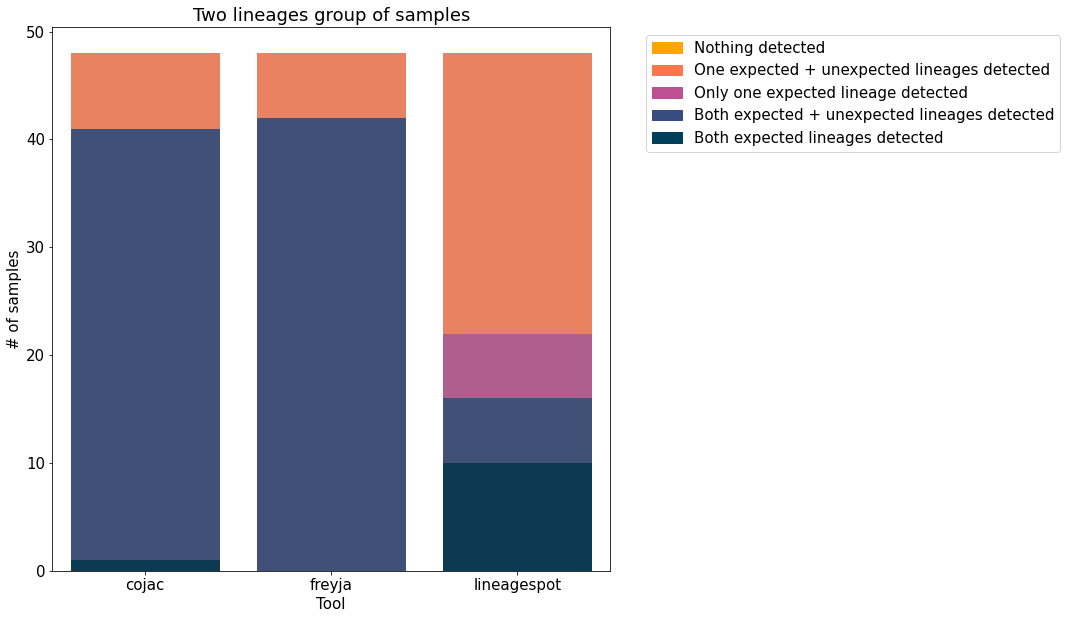
\includegraphics[width=0.8\textwidth]{figures/results/mock/twolin-num-bars.png}
                \captionof{figure}{Bar plot describing the number of mock samples of two lineages group that meet one of five characteristics: i) both expected lineages detected; ii) only one expected lineage detected; iii) one expected plus unexpected lineages detected; iv) both expected plus unexpected lineages detected; v) nothing detected.}
                \label{fig:results:mock:bar-twolin}
            \end{figure}
                \subparagraph{Barplot}
                According to \cref{fig:results:mock:bar-twolin}, overall, 48 samples are in Two lineages group. From the bar plot, it is obvious that all three tools are effective in detecting both expected lineages. Nonetheless, in the detection of only two expected lineages and nothing more. Lineagespot performed the best, compared to COJAC and Freyja, as it is the only tool that was able to detect 10 samples out of 48 with two expected lineages and nothing more. As was already shown for the Single lineage group, Freyja is effective at detecting expected lineages (in 42 samples out of 48); however, it always detected some unexpected lineages. COJAC's results for two lineages are considerably close to Freyja's results; they both detected around 40 samples with two lineages expected. Even more, in one sample, COJAC was able to detect only expected lineages. Interestingly, no tools detected nothing for this group of samples.

                \subparagraph{Venn Upset}
                Venn Upset diagram below (\cref{fig:results:mock:venn-twolin}) was constructed based on 48 samples in which there were two lineages expected. Each column corresponds to a set of obtained results of certain tools (COJAC, Lineagespot, Freyja), and bar charts on top show the size of the set of tool’s results. The first row in the figure is completely empty, while 3 samples are expected to be detected but were not. These three samples are distinct from other samples by belonging to the “low coverage” group. In addition, there are a few samples in which 2 expected lineages were detected by only one tool: 1,2, and 3 samples corresponding to Lineagespot, Freyja, and COJAC. At the same time, Freyja and COJAC detected two expected lineages in 24 same samples, whereas Lineagespot did not detect both expected lineages, so there is no interaction with Lineagespot set here, but there is one between Freyja and COJAC. That can be explained by the same workflow used for Freyja and COJAC results but the different method used by Lineagespot pipeline. Interestingly, all three tools Lineagespot, Freyja, and COJAC detected the expected two lineages in 15 same samples.
                \begin{figure}[ht!]
                	\centering
                    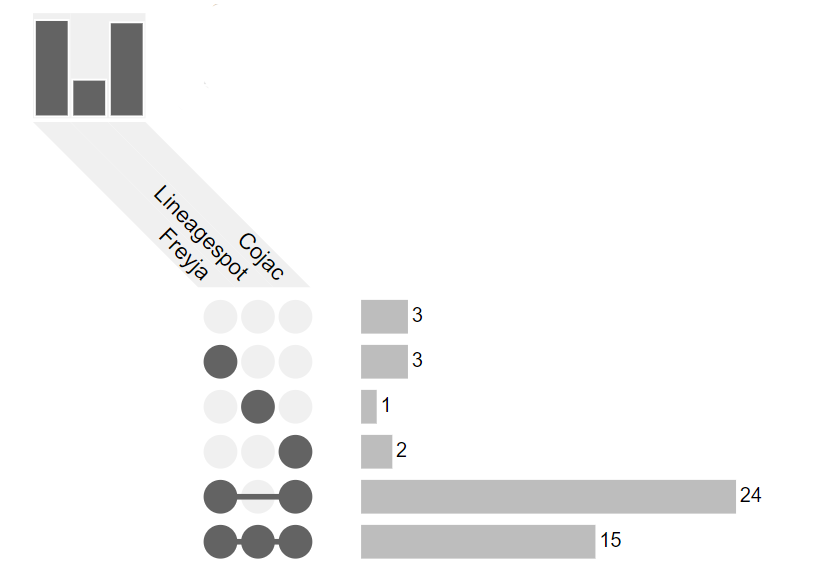
\includegraphics[width=0.7\textwidth]{figures/results/mock/venn-twolin.png}
                    \captionof{figure}{Venn Upset diagram constructed based on 48 samples of the synthetic mock dataset in which there were two lineages expected.}
                    \label{fig:results:mock:venn-twolin}
                \end{figure}
                \subparagraph{Barplots: proportion comparison}
                In cases: i) both expected lineages detected and ii) both expected + unexpected lineages detected, there were additionally 6 bar plots generated to evaluate if expected proportion between two expected lineages is correctly defined by different tools. Proportions between expected lineages that were considered are: i) BA1 > BA2; ii) BA1 = BA2; iii) BA1 < BA2; iv) BA1 > Delta;  v) BA1 = Delta; vi) BA1 < Delta. These plots show every case where this proportion was expected (one plot per 1 of 6 cases), and the corresponding results from Freyja, COJAC, and Lineagespot are plotted in \cref{fig:results:mock:ba1-ba2} and \cref{fig:results:mock:ba1-delta}.
                \begin{figure}[H]
                    \begin{subfigure}{\linewidth}
                	\centering
                    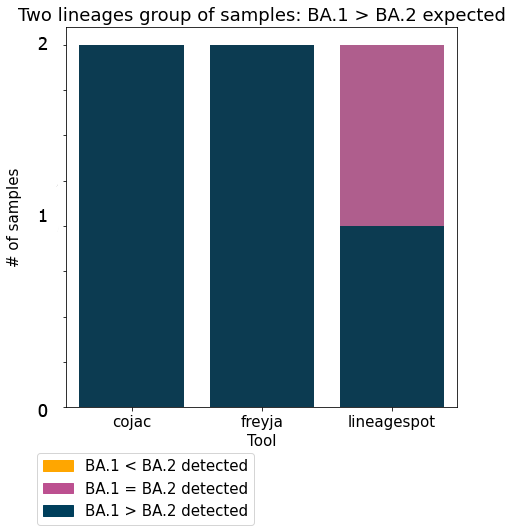
\includegraphics[width=0.3\textwidth]{figures/results/mock/ba1Gba2-bars.png}\hfill
                    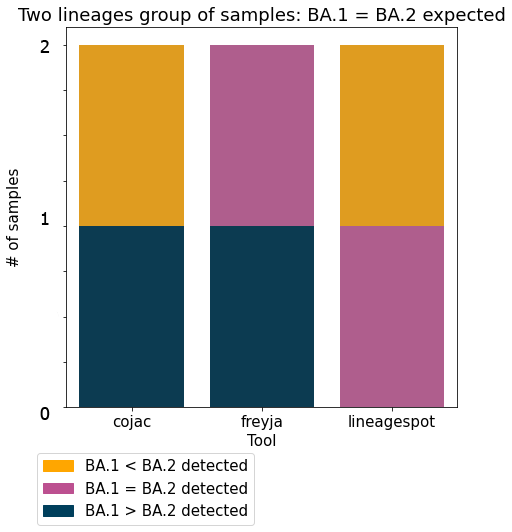
\includegraphics[width=0.3\textwidth]{figures/results/mock/ba1EQba2-bars.png}\hfill
                    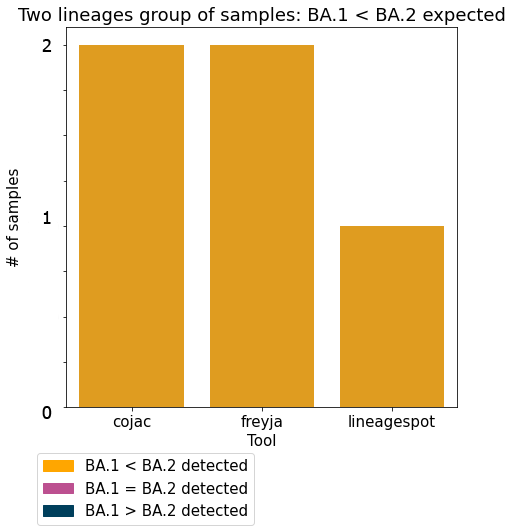
\includegraphics[width=0.3\textwidth]{figures/results/mock/ba1Lba2-bars.png}
                    \captionof{figure}{Bar plots for "two lineages" group of mock samples where following proportions were expected: i) BA1 > BA2; ii) BA1 = BA2; iii) BA1 < BA2.}
                    \label{fig:results:mock:ba1-ba2}
                    \end{subfigure}\par\medskip
                    \begin{subfigure}{\linewidth}
                	\centering
                    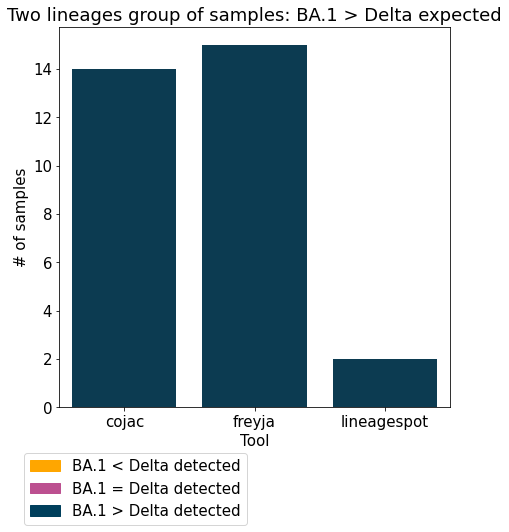
\includegraphics[width=0.3\textwidth]{figures/results/mock/ba1Gd-bars.png}\hfill
                    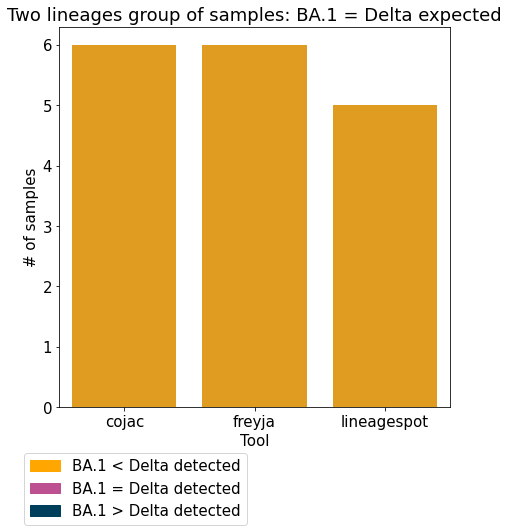
\includegraphics[width=0.3\textwidth]{figures/results/mock/ba1EQd-bars.png}\hfill
                    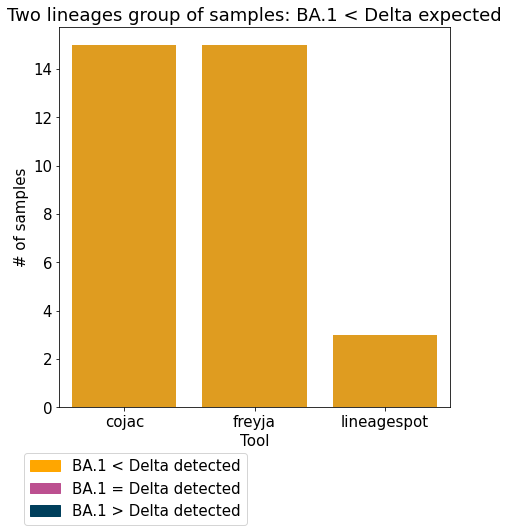
\includegraphics[width=0.3\textwidth]{figures/results/mock/ba1Ld-bars.png}
                    \captionof{figure}{Bar plots for "two lineages" group of mock samples where following proportions were expected: iv) BA1 > Delta; v) BA1 = Delta; vi) BA1 < Delta.}
                    \label{fig:results:mock:ba1-delta}
                    \end{subfigure}\par\medskip
                \end{figure}
                
                For the “two lineages” expected group of samples, there are only 6 samples where BA.1 and BA.2 lineages were expected together \cref{fig:results:mock:ba1-ba2}): 2 for every type of proportion. For the case, when the proportion of BA.1 > BA.2 is expected, both COJAC and Freyja detected the same proportion between these two lineages, while Lineagespot only in 1 sample. In case of equal presence of BA.1 and BA.2 in samples, Freyja and Lineagespot detected 1 sample against 2 expected. In the case of BA.1 < BA.2, all tools detected samples correctly, however, Lineagesspot detected only 1 out of 2. 

                For the “two lineages” expected group of samples, there are 42 samples where BA.1 and Delta lineages were expected together (\cref{fig:results:mock:ba1-delta}): 18 for BA.1 > Delta type of relation between lineage proportions, 6 for BA.1 = Delta, and 18 samples for BA.1 < Delta. For the case when the proportion of BA.1 > Delta is expected, all tools detected it correctly but not in all 18 samples. However, Freyja and COJAC performed well, being able to detect 15 and 14 samples with this type of relation, respectively. Lineagespot detected only 2 samples. Likewise, for the case of BA.1 < Delta all tools detected some samples but not all expected samples, Freyja and COJAC both detected 15 out of 18 which is significantly more than Lineagespot with its 3. Finally, when BA.1 = Delta was the expected relation, all tools discerned BA.1 < Delta relation.

        \subsubsection{Benchmarking Freyja- and COJAC- based workflow results}
        \paragraph{Distribution: linages proportions among tools}
        To compare Freyja and COJAC branches of workflow in another way, and to assess results with expected ones, in \cref{fig:results:mock:dist-delta-all}, \ref{fig:results:mock:dist-ba1-all}, and \ref{fig:results:mock:dist-ba1-all}, taking all 100 samples into account, the distributions of every lineage (Delta, BA.1, BA.2) are shown among received results from Freyja, COJAC, and expected proportions. It is seen that for Delta and BA.1 lineages of SARS-CoV-2 there is quite a similar number of samples carrying the same proportion of the considered lineage. Interestingly, for all lineages smaller number of samples with a low proportion of lineage was expected than detected by tools Freyja and COJAC. For BA.1 lineage there were expected more samples with higher lineage proportion than was found by Freyja and COJAC. 
        \begin{figure}[H]
            \centering
            \begin{subfigure}[b]{0.3\textwidth}
            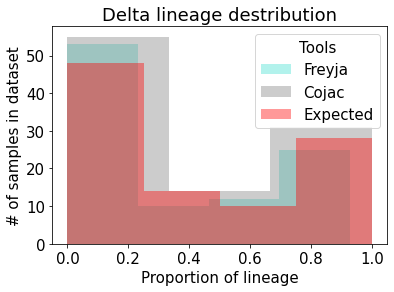
\includegraphics[width=1\textwidth]{figures/results/mock/distr-delta.png}
            \captionof{figure}{Delta}
            \label{fig:results:mock:dist-delta-all}
            \end{subfigure}
            \hfill
            \begin{subfigure}[b]{0.3\textwidth}
            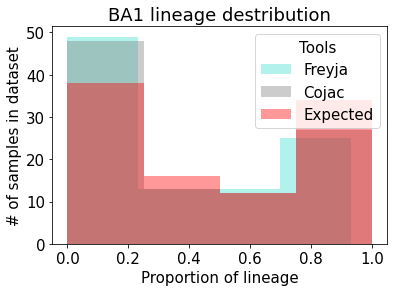
\includegraphics[width=1\textwidth]{figures/results/mock/distr-ba1.png}
            \captionof{figure}{BA.1}
            \label{fig:results:mock:dist-ba2-all}
            \end{subfigure}
            \hfill
            \begin{subfigure}[b]{0.3\textwidth}
            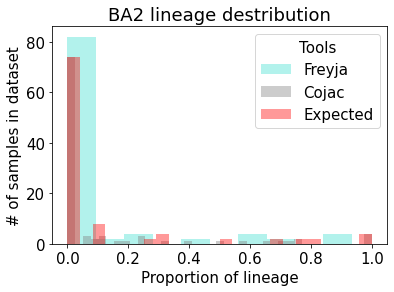
\includegraphics[width=1\textwidth]{figures/results/mock/distr-ba2.png}
            \captionof{figure}{BA.2}
            \label{fig:results:mock:dist-ba1-all}
            \end{subfigure}
            \captionof{figure}{The lineage proportion distribution among results from Freyja, COJAC on mock dataset (all samples), compared with expected proportions.}
        \end{figure}
        
        \paragraph{Distribution: tools results among all mock samples}
        The other angle to observe results and compare them, is to look at how lineages are distributed in results produced by every tool. In \cref{fig:results:mock:dist-freyja-all}, one can see that Freyja detected BA.2 with a small presence in most of the samples (around 80 out of 100), while Delta and BA.1 were found by Freyja in more or less similar proportions. Looking at \cref{fig:results:mock:dist-cojac-all}, one can see just a bit different distribution when most of the samples contained a very small proportion of BA.2 according to COJAC results. In both graphs, Delta and BA.1 lineages were found in small proportion, before 0.3, in around half of samples, while around 20-30\% of samples carry Delta and BA.1 in high presence, from 0.7 to 1 value of the proportion of lineage abundance.
        
        \begin{figure}[H]
            \centering
            \begin{subfigure}[b]{0.45\textwidth}
            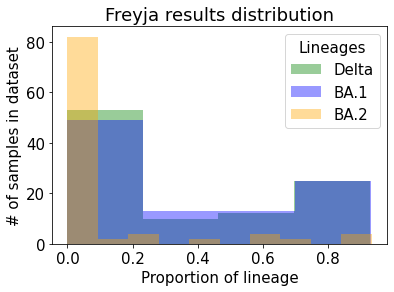
\includegraphics[width=1\textwidth]{figures/results/mock/distr-freyja.png}
            \captionof{figure}{Freyja}
            \label{fig:results:mock:dist-freyja-all}
            \end{subfigure}
            \hfill
            \begin{subfigure}[b]{0.45\textwidth}
            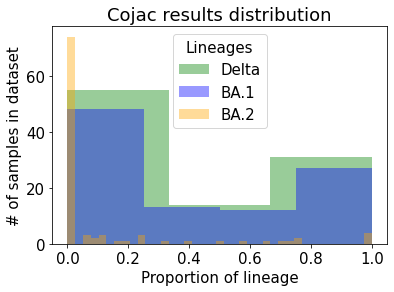
\includegraphics[width=1\textwidth]{figures/results/mock/distr-cojac.png}
            \captionof{figure}{COJAC}
            \label{fig:results:mock:dist-cojac-all}
            \end{subfigure}
            \captionof{figure}{All three considered lineages (Delta, BA.1, BA.2) proportion distribution among results from the tool on mock dataset.}
        \end{figure}
        
    
    \subsection{Real-world datasets results} \label{sec:results:real}
    For this thesis, the real-world data for experiments were chosen based on the principle that samples were collected over a variety of time periods and locations around the world. In chosen four datasets, I aimed to cover these principles expecting to observe evolution of SARS-CoV-2 over time as well as to show variations in prevalence of a variety of SARS-CoV-2 lineages depending on the location.

    Metadata on real-world datasets of choice for this master thesis is shown in \cref{tab:methods:real-datasets}. In the following sections, the results of running developed Galaxy workflows will be shown. \Cref{sec:results:real:california} will represent results of Freyja-based Galaxy workflow on the Californian dataset, \cref{sec:results:real:canada} - Freyja-based and COJAC-based workflows results on the Canadian dataset, \cref{sec:results:real:us} - Freyja-based and COJAC-based workflows results on US dataset, and, finally, \cref{sec:results:real:uk} - Freyja-based and COJAC-based workflows results on UK dataset. 

    \subsubsection{Dataset (PRJNA661613): California sewage metatranscriptomes enriched for respiratory viruses} \label{sec:results:real:california}
    For this dataset, samples of raw sewage were collected from wastewater treatment facilities in Alameda and Marin Counties in Northern California between 13 May 2020 and 30 July 2020 at a wastewater interceptor (labeled Berkeley, Berkeley Hills, Oakland, and Marin, according to the municipal areas each serves).

    For this dataset, only the Freyja-based branch of Galaxy workflow was launched because the COJAC-based branch is applicable only to the ampliconic library preparation dataset, while Freyja can work with metatranscriptomics which is the case of the Californian dataset.
    
    In the step of checking the abundance of other species that are unmapped to reference SARS-CoV-2 sequence on the Californian dataset, Kraken2 was run on a dataset collection using viral genomes taxa database, following Krona pie charts generation. Going across samples’, approximately 78\% to around 85\% of fragments are covered by the clade rooted at unclassified taxon. In a similar manner, from sample to sample percentage, from around 18\% to 22\%, of fragments are covered by the clade rooted at either viruses, ribovirus, nidovirales, cornidovirineae, or coronaviridae taxon. Slightly smaller proportions of fragments are covered by the clade rooted at Orthocoronavirinae, Betacoronavirus, Sarbecovirus, Severe acute respiratory syndrome-related coronavirus, and SARS coronavirus, around 12-15\%. Notable, the number of fragments assigned directly to the SARS coronavirus taxon is non-zero, as it is for most of the taxons. 
    
    Krona charts were produced for every sample separately, followed by a Krona pie that represents all samples in one pie chart. \Cref{fig:results:real:krona-sf-a}, \ref{fig:results:real:krona-sf-b} show resulting examples of Krona charts for two separate samples (SRR12596166 and SRR12596175, respectively), \cref{fig:results:real:krona-sf-c} illustrates Krona pie for aggregated all samples of dataset. 
    
    \begin{figure}[H]
        \centering
        \begin{subfigure}[b]{0.45\textwidth}
        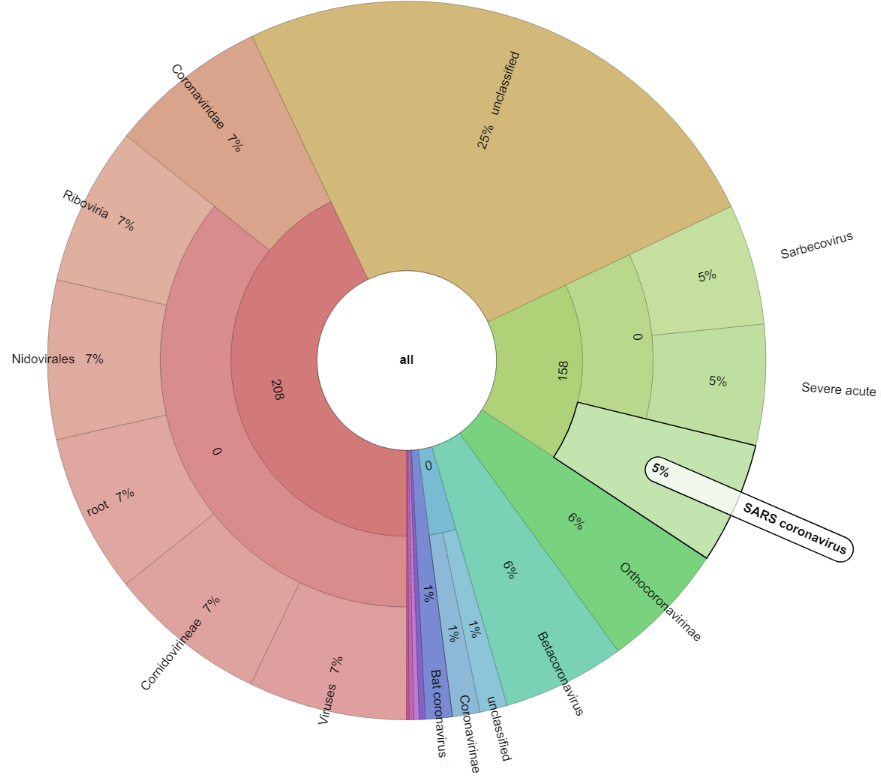
\includegraphics[width=1\textwidth]{figures/results/real/krona/krona-sf-sSRR12596166.png}
        \captionof{figure}{Krona for sample SRR12596166}
        \label{fig:results:real:krona-sf-a}
        \end{subfigure}
        \hfill
        \begin{subfigure}[b]{0.43\textwidth}
        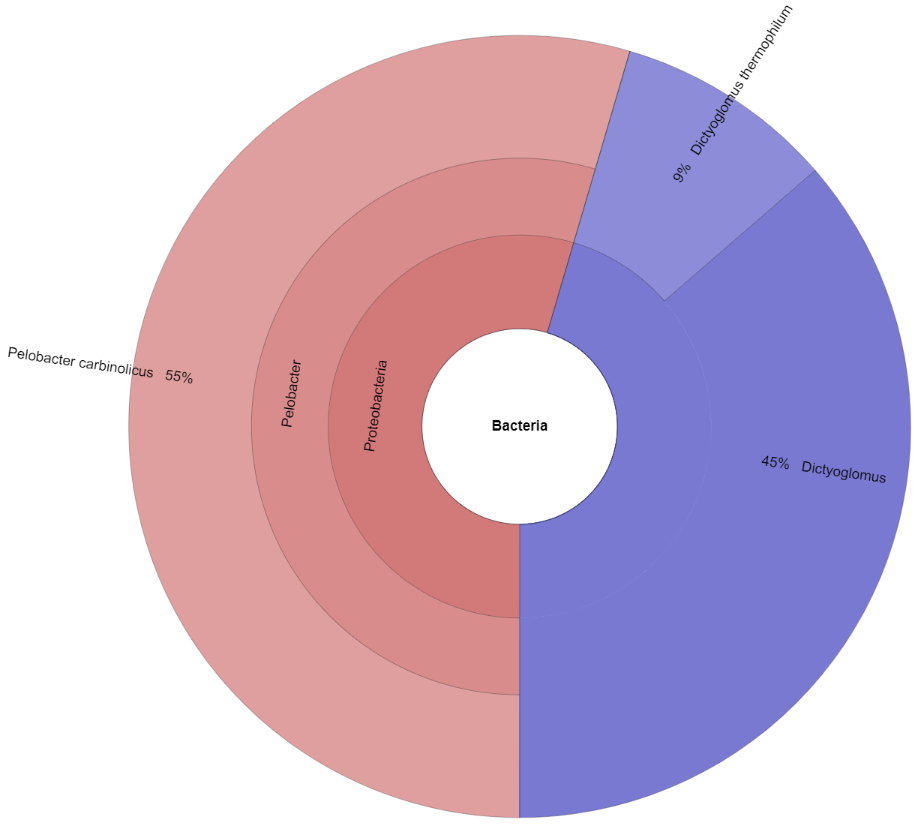
\includegraphics[width=1\textwidth]{figures/results/real/krona/krona-sf-sSRR12596175.png}
        \captionof{figure}{Krona for sample SRR12596175}
        \label{fig:results:real:krona-sf-b}
        \end{subfigure}
        \hfill
        \begin{subfigure}[b]{0.45\textwidth}
        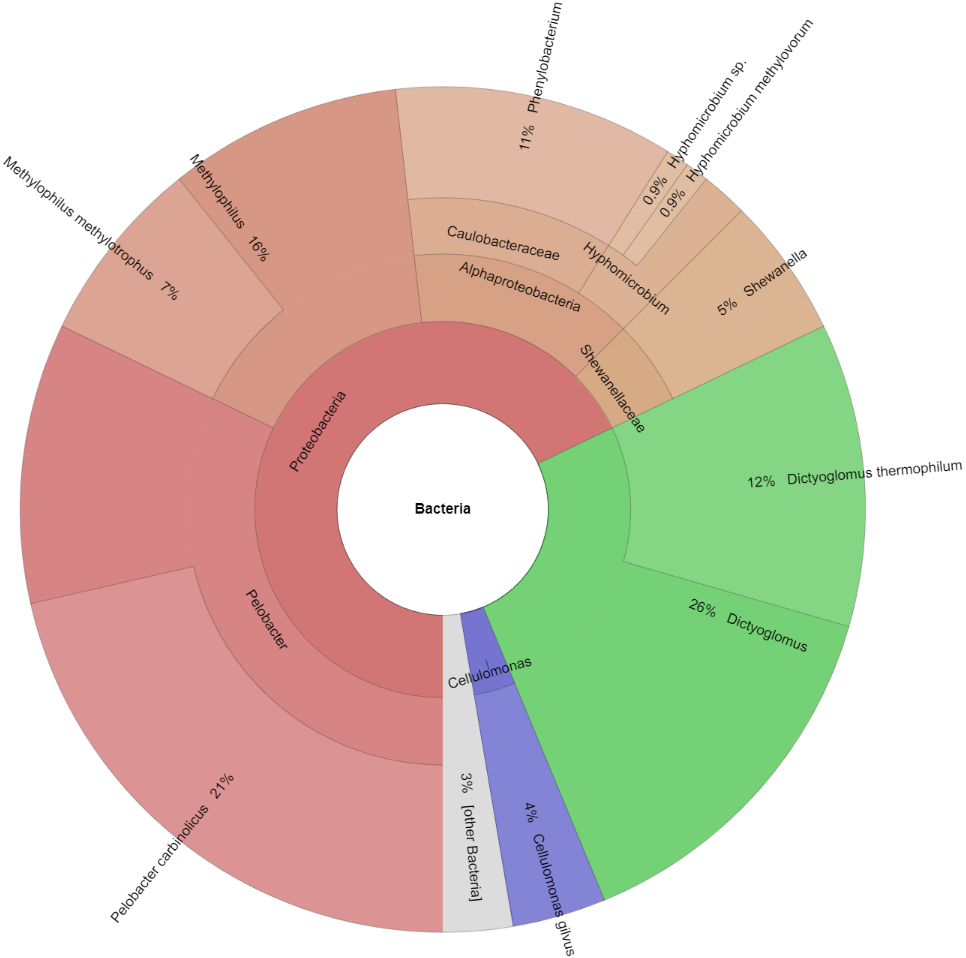
\includegraphics[width=1\textwidth]{figures/results/real/krona/krona-sf-all.png}
        \captionof{figure}{Krona for all aggregated samples}
        \label{fig:results:real:krona-sf-c}
        \end{subfigure}
        \captionof{figure}{Krona chart visualizing the abundances of species in wastewater samples from the Californian dataset (PRJNA661613).}
    \end{figure}
    
    As for lineages abundances analysis on the Californian dataset, there were no exact names, like Omicron, Delta, etc., defined by Freyja using UShER bar-codes. So, for aggregation tables and for plotting Freyja used the label “Other” (see \cref{tab:appendix:freyja} in \cref{sec:appendix:tabs:freyja}). When detecting lineages that are considered by Freyja as “Other” designated name, the result bar plots are non-informative since they contain only one group of lineage - “Other”. Moreover, trying to produce an interactive dashboard, Freyja can meet an issue with “too many lineages to plot”. Due to Freyja's limitations, for the Californian dataset, plots were either non-informative or not generated.
    
    \subsubsection{Dataset (PRJNA824537): Wastewater influents from wastewater treatment facilities across Ontario, Canada} \label{sec:results:real:canada}
    Wastewater samples were collected by Canadian Research Institute for Food Safety. The dataset contains one of the relatively recent samples, the last sample was published in June of 2022.

    Similarly to the Californian dataset analysis, Krona charts were created for each sample of the Canadian dataset separately, followed by a Krona pie representing all samples. \Cref{fig:results:real:krona-ca-a}, \ref{fig:results:real:krona-ca-b} show resulting examples of Krona charts for two separate samples (SRR18680446 and SRR18680489, respectively), \cref{fig:results:real:krona-ca-c} illustrates Krona pie for aggregated all samples of dataset.
    \begin{figure}[H]
        \centering
        \begin{subfigure}[b]{0.46\textwidth}
        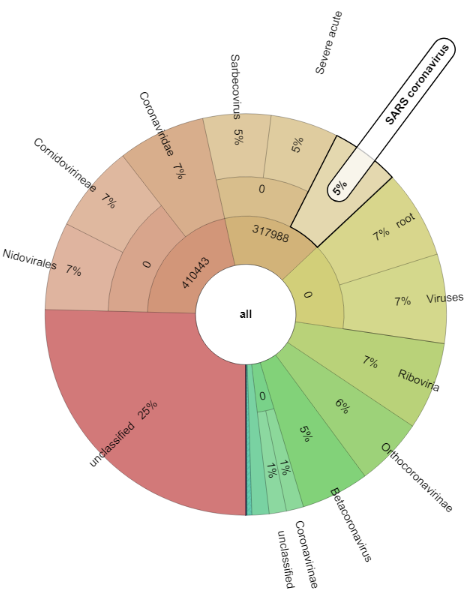
\includegraphics[width=1\textwidth]{figures/results/real/krona/krona-ca-sSRR18680446.png}
        \captionof{figure}{Krona for sample SRR18680446}
        \label{fig:results:real:krona-ca-a}
        \end{subfigure}
        \hfill
        \begin{subfigure}[b]{0.44\textwidth}
        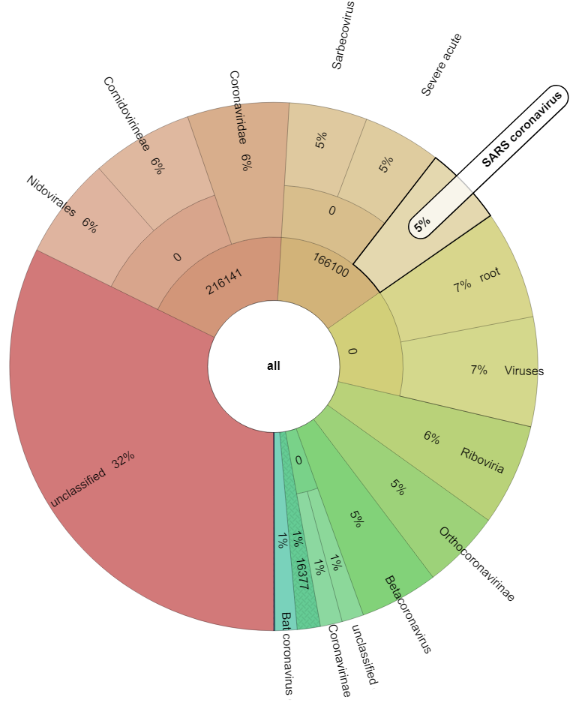
\includegraphics[width=1\textwidth]{figures/results/real/krona/krona-ca-sSRR18680489.png}
        \captionof{figure}{Krona for sample SRR18680489}
        \label{fig:results:real:krona-ca-b}
        \end{subfigure}
        \hfill
        \begin{subfigure}[b]{0.44\textwidth}
        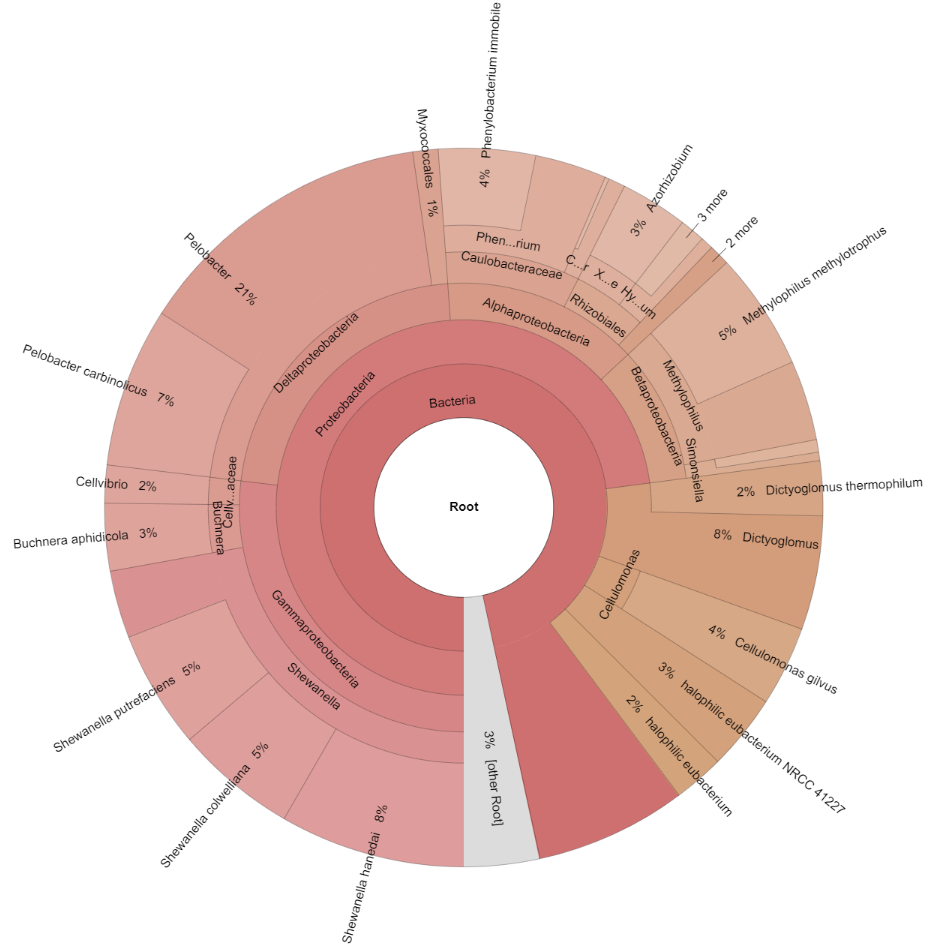
\includegraphics[width=1\textwidth]{figures/results/real/krona/krona-ca-all.png}
        \captionof{figure}{Krona for all aggregated samples}
        \label{fig:results:real:krona-ca-c}
        \end{subfigure}
        \captionof{figure}{Krona chart visualizing the abundances of species in wastewater samples from the Canadian dataset (PRJNA824537).}
    \end{figure}
    
    Regarding results on SARS-CoV-2 lineages abundances, for the dataset from Ontario, Canada (PRJNA824537), there were readable plots generated by Freyja (\cref{fig:results:real:ca-freyja-samples},\ref{fig:results:real:ca-freyja-daily}). In \cref{fig:results:real:ca-freyja-samples}, one can see all samples represented by bars (one bar per sample). However, they are not in order of collecting date and time, which makes it difficult to interpret. One can see that some of the samples contain abundant Omicron lineage, and some other samples have abundant Delta. Nevertheless, it is the general picture of lineages abundance among samples. \Cref{fig:results:real:ca-freyja-daily}, in contrast, represents trends and changes in lineage abundances over time. Delta was a prevalent lineage at the beginning of December 2021, while from the mid of December 2021, Omicron began to be most predominant, and its abundance increased significantly up to around 0.9 lineage abundance proportion in February 2022. It's worth noting that Freyja always detected other lineages in samples, except Omicron and Delta, although in small proportions, around 0.05.
    
    \begin{figure}[H]
        \centering
        \begin{subfigure}[b]{1\textwidth}
        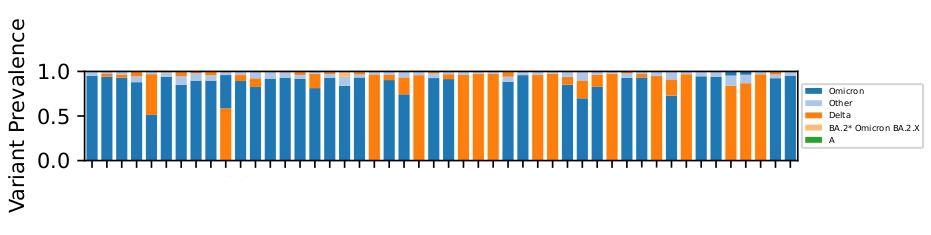
\includegraphics[width=1\textwidth]{figures/results/real/ca-freyja-samples.png}
        \captionof{figure}{Variant prevalence across samples.}
        \label{fig:results:real:ca-freyja-samples}
        \end{subfigure}
        \hfill
        \begin{subfigure}[b]{0.8\textwidth}
        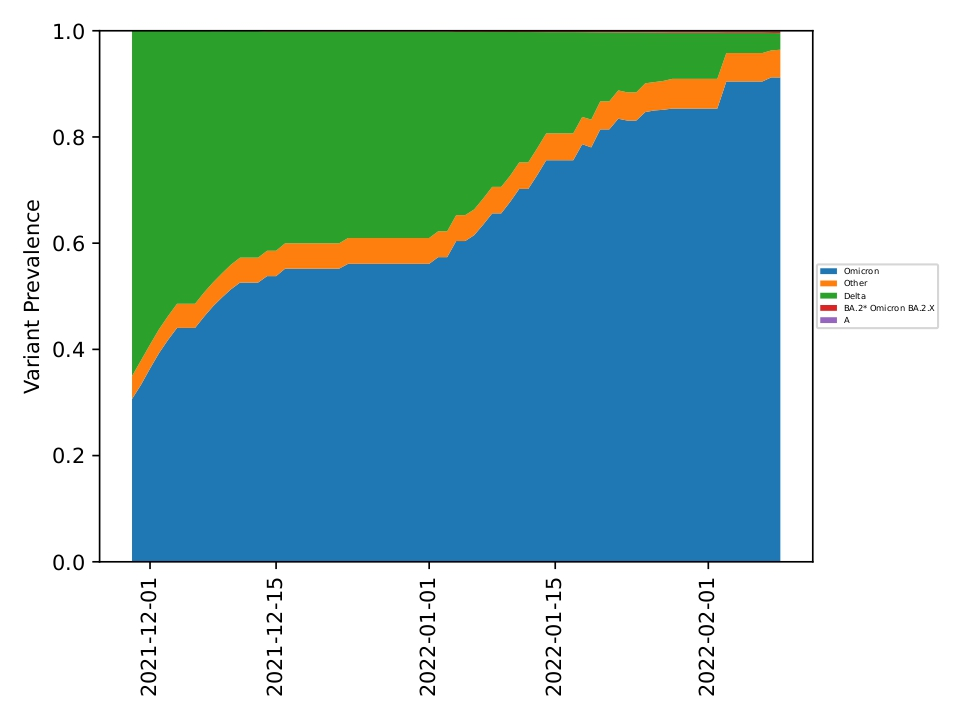
\includegraphics[width=1\textwidth]{figures/results/real/ca-freyja-daily.jpg}
        \captionof{figure}{Variant prevalence with daily binning.}
        \label{fig:results:real:ca-freyja-daily}
        \end{subfigure}
        \hfill
        \captionof{figure}{Variant prevalence computed by Freyja over samples, produced by Freyja on Ontario, Canada (PRJNA824537).}
    \end{figure}
    
    To compare results on the Canadian (PRJNA824537) dataset from both Freyja and COJAC branches of Galaxy workflow, two bar plots were considered: one generated by Freyja (\cref{fig:results:real:ca-freyja-monthly}), one generated from COJAC results using Matplotlib Python library with the same color scheme (\cref{fig:results:real:ca-cojac-monthly}). 
    
    \begin{figure}[H]
        \centering
        \begin{subfigure}[b]{0.6\textwidth}
        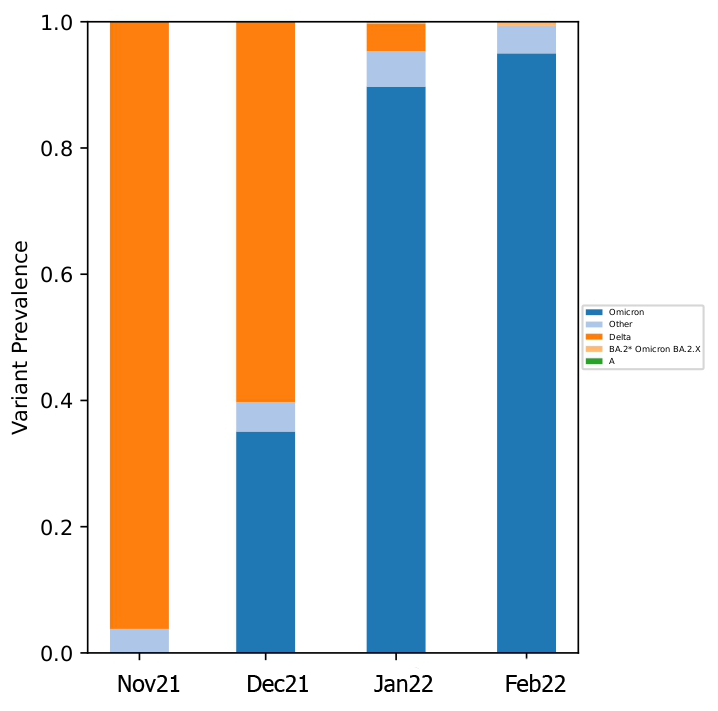
\includegraphics[width=1\textwidth]{figures/results/real/ca-freyja-monthly.png}
        \captionof{figure}{Bar plot generated by Freyja.}
        \label{fig:results:real:ca-freyja-monthly}
        \end{subfigure}
        \hfill
        \begin{subfigure}[b]{0.7\textwidth}
        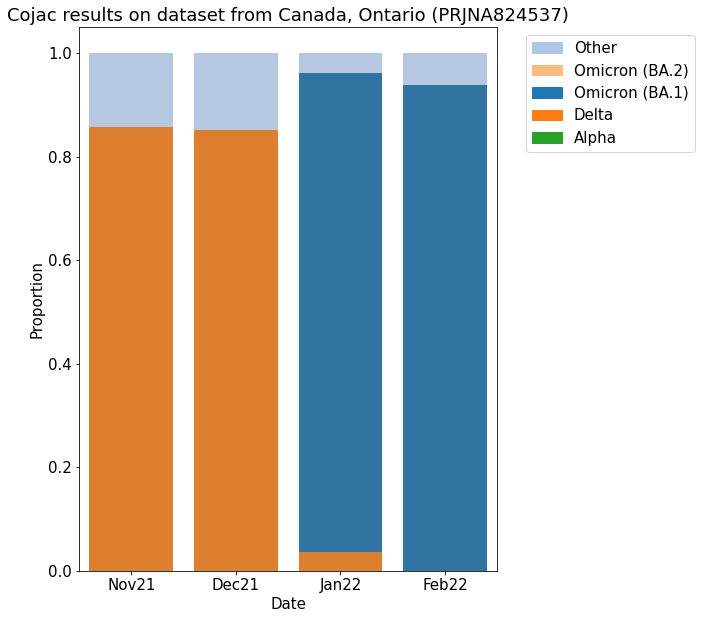
\includegraphics[width=1\textwidth]{figures/results/real/ca-cojac-monthly.png}
        \captionof{figure}{Bar plot generated from COJAC output using Python.}
        \label{fig:results:real:ca-cojac-monthly}
        \end{subfigure}
        \hfill
        \captionof{figure}{Bar plot with sample collection time information grouped by month, for the Canadian (PRJNA824537) dataset.}
    \end{figure}
    
    Results on the Canadian (PRJNA824537) dataset from Freyja and COJAC differ, as shown in \cref{fig:results:real:ca-freyja-monthly}, \ref{fig:results:real:ca-cojac-monthly}. However, the prevalence of Delta in November and December 2021 and the prevalence of Omicron in January and February 2022 are discerned by both methods. Another interesting observation is that Freyja found the Omicron variant already in December 2021, while COJAC was able to detect Omicron only in January 2022.
    
    \subsubsection{Dataset (PRJNA765346): GenomeTrakr wastewater project of Washington State Department of Health, US} \label{sec:results:real:us}
    Samples for this dataset were and are being collected by the FDA Center for Food Safety and Applied Nutrition. This dataset is one of the most extensive dataset with more than 400 samples so far, and regularly new samples are being added (the last samples being from October of 2022). This dataset is of research interest also because it can be considered in the future as one of those that will be regularly analyzed by the Galaxy bot that was described in \cref{sec:intro:galaxy-effort}.

    Similarly to the Californian and Canadian datasets, Krona charts were created for each sample of the US dataset separately, followed by a Krona pie representing all samples. \Cref{fig:results:real:krona-us-a}, \ref{fig:results:real:krona-us-b}, and \ref{fig:results:real:krona-us-c} show resulting examples of Krona charts for three separate samples (SRR17578350, SRR18300811, and SRR20997582, respectively). Krona cheat generated for all combined datasets is too abundant and rather non-informative to show.
    
    \begin{figure}[H]
        \centering
        \begin{subfigure}[b]{0.45\textwidth}
        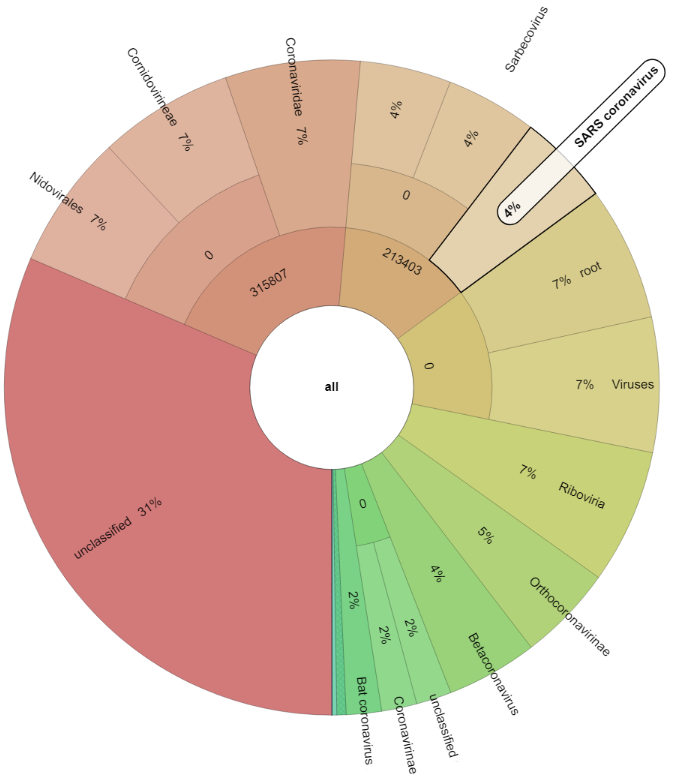
\includegraphics[width=1\textwidth]{figures/results/real/krona/krona-us-sSRR17578350.png}
        \captionof{figure}{Krona for sample SRR17578350}
        \label{fig:results:real:krona-us-a}
        \end{subfigure}
        \hfill
        \begin{subfigure}[b]{0.45\textwidth}
        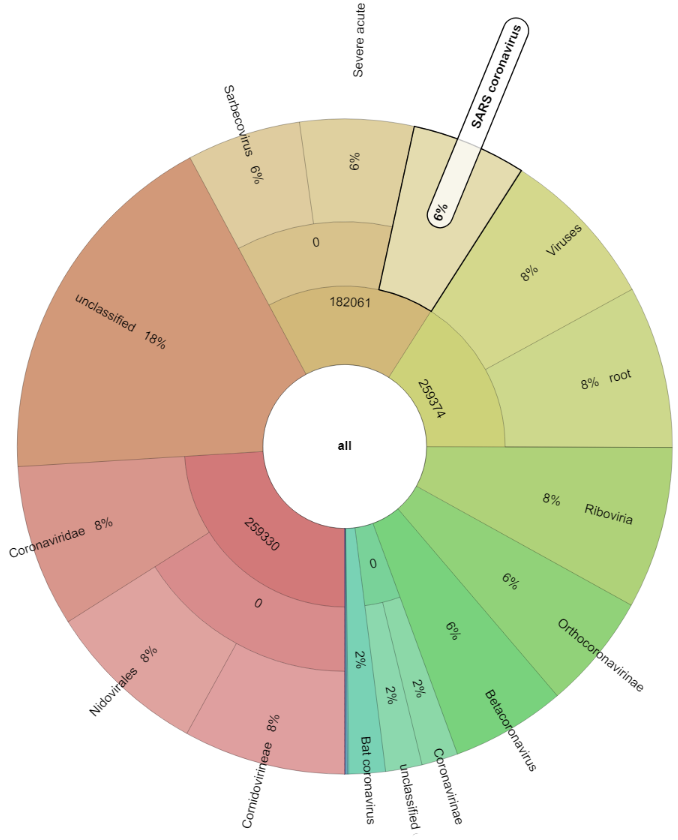
\includegraphics[width=1\textwidth]{figures/results/real/krona/krona-us-sSRR18300811.png}
        \captionof{figure}{Krona for sample SRR18680489}
        \label{fig:results:real:krona-us-b}
        \end{subfigure}
        \hfill
        \begin{subfigure}[b]{0.47\textwidth}
        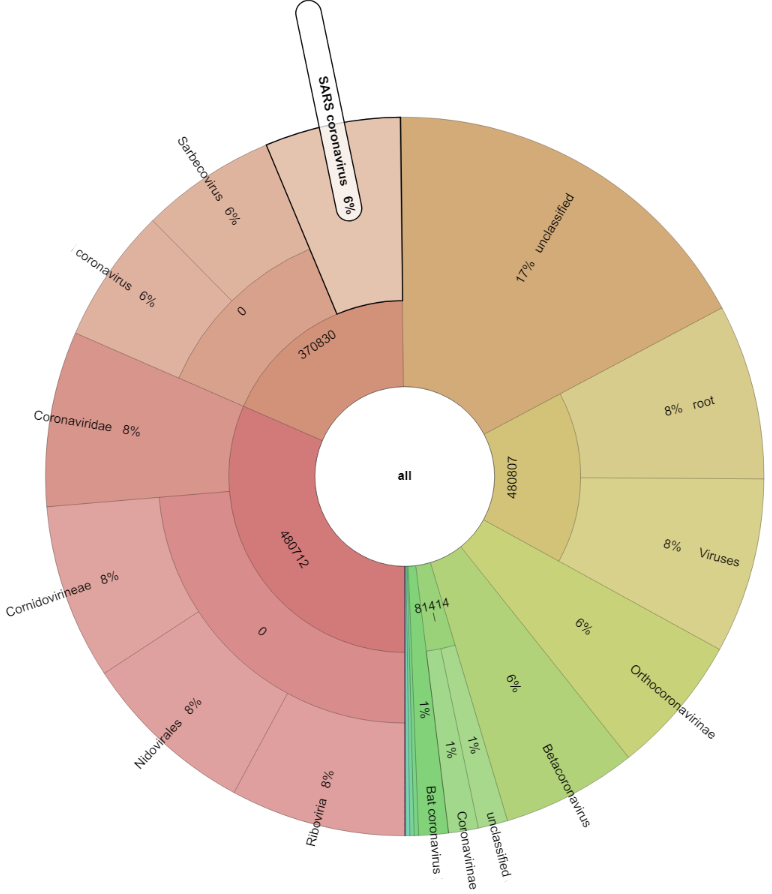
\includegraphics[width=1\textwidth]{figures/results/real/krona/krona-us-sSRR20997582.png}
        \captionof{figure}{Krona for sample SRR20997582}
        \label{fig:results:real:krona-us-c}
        \end{subfigure}
        \captionof{figure}{Krona chart visualizing the abundances of species in wastewater samples from the US dataset (PRJNA765346).}
    \end{figure}
    
    As for results on lineage abundances received for the US (PRJNA765346) dataset, the distribution of SARS-CoV-2 lineages over time binned by the day, obtained in Freyja-based branch of the workflow, is depicted in \cref{fig:results:real:us-freyja-daily}.
    
    \begin{figure}[ht!]
        \centering
        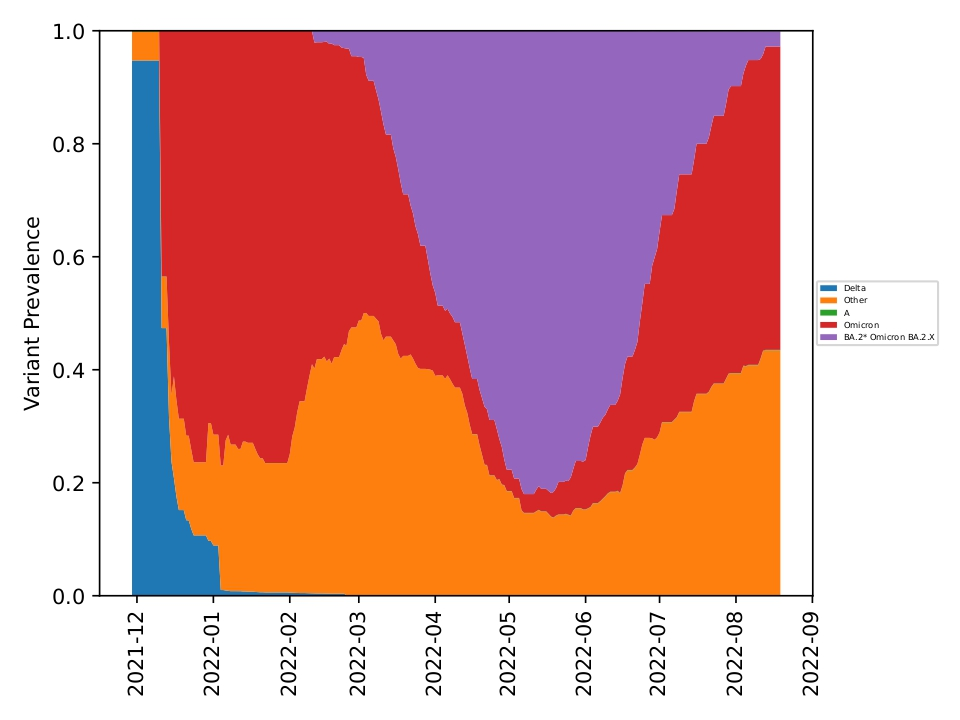
\includegraphics[width=0.9\textwidth]{figures/results/real/us-freyja-daily.jpg}
        \captionof{figure}{Smooth plot with sample collection time information with daily binning for US (PRJNA765346) dataset.}
        \label{fig:results:real:us-freyja-daily}
    \end{figure}
    
    \Cref{fig:results:real:us-freyja-daily} shows curious results. Delta was found by Freyja in samples of the US dataset only in November 2021. From January to March 2022, Omicron (BA.1 sub-lineage) was prevalent, accompanied by other lineages found in samples but grouped into “Other” lineages. From April to June 2022, the BA.2 sub-lineage of Omicron was common in the US dataset. Finally, by September 2022, Omicron BA.1 took the prevalence back, with about 0.6 proportion against 0.4 for other lineages.

    To compare results on the US (PRJNA765346) dataset from both Freyja and COJAC branches of Galaxy workflow, there were two bar plots created: one was generated by Freyja  (\cref{fig:results:real:us-freyja-monthly}), while the other was generated from COJAC results using Matplotlib Python library with the same color scheme (\cref{fig:results:real:us-cojac-monthly})).
    
    \begin{figure}[H]
        \centering
        \begin{subfigure}[b]{1\textwidth}
        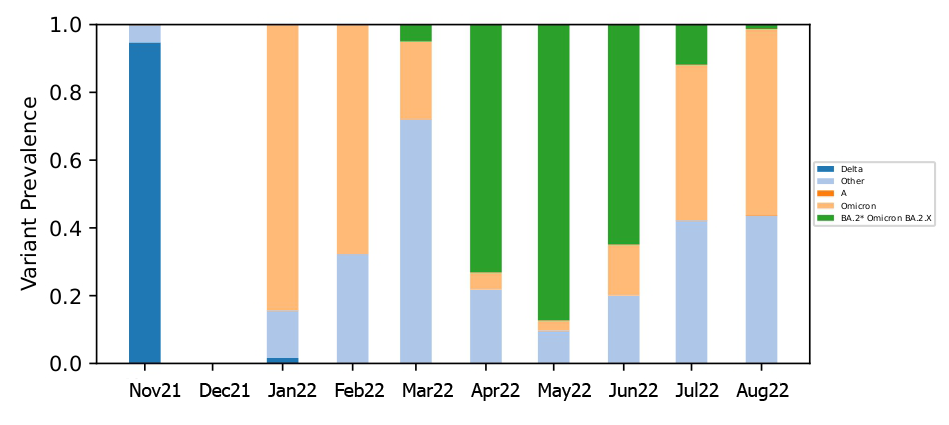
\includegraphics[width=1\textwidth]{figures/results/real/us-freyja-monthly.png}
        \captionof{figure}{Bar plot generated by Freyja.}
        \label{fig:results:real:us-freyja-monthly}
        \end{subfigure}
        \hfill
        \begin{subfigure}[b]{0.9\textwidth}
        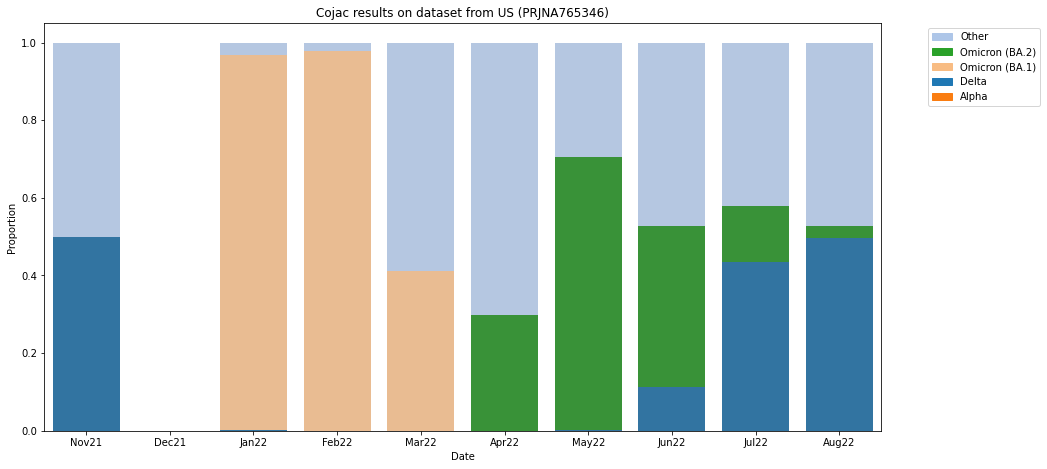
\includegraphics[width=1\textwidth]{figures/results/real/us-cojac-monthly.png}
        \captionof{figure}{Bar plot generated from COJAC output using Python.}
        \label{fig:results:real:us-cojac-monthly}
        \end{subfigure}
        \hfill
        \captionof{figure}{Bar plot with sample collection time information grouped by month, for US (PRJNA765346) dataset.}
    \end{figure}
    
    Results from Freyja and COJAC on the US dataset are obviously not the same. The curious fact is detecting the considerable prevalence of the Delta lineage in summer 2022 by COJAC and not detecting it by Freyja. And more expected that both tools found Delta at the end of 2021 and the prevalence of Omicron (both BA.1 and BA.2 sub-lineages) in 2022. Interestingly, the BA.1 lineage was prevalent from January to March 2022, while BA.2 from April to June 2022.
    
    \subsubsection{Dataset (PRJEB42191): monitoring SARS-CoV-2 in municipal wastewater in the UK} \label{sec:results:real:uk}
    Samples for this dataset were collected from six wastewater treatment plants located in Wales and Northwest England. The treatment plants served urban areas in Gwynedd, Cardiff, Liverpool, Manchester, the Wirral and Wrexham, with a combined population equivalent to 3 million people. Weekly samples of untreated wastewater influent were taken from the six treatment plants between March and June 2020.
    
    Similarly to the Californian, Canadian, and US datasets, Krona charts were created for each sample of the UK dataset separately, followed by a Krona pie representing all samples. \Cref{fig:results:real:krona-uk-a}, \ref{fig:results:real:krona-uk-b} show resulting examples of Krona charts for two separate samples (ERR5014633 and ERR5014683, respectively), \cref{fig:results:real:krona-ca-c} illustrates Krona pie for aggregated all samples of dataset.
    
    \begin{figure}[H]
        \centering
        \begin{subfigure}[b]{0.42\textwidth}
        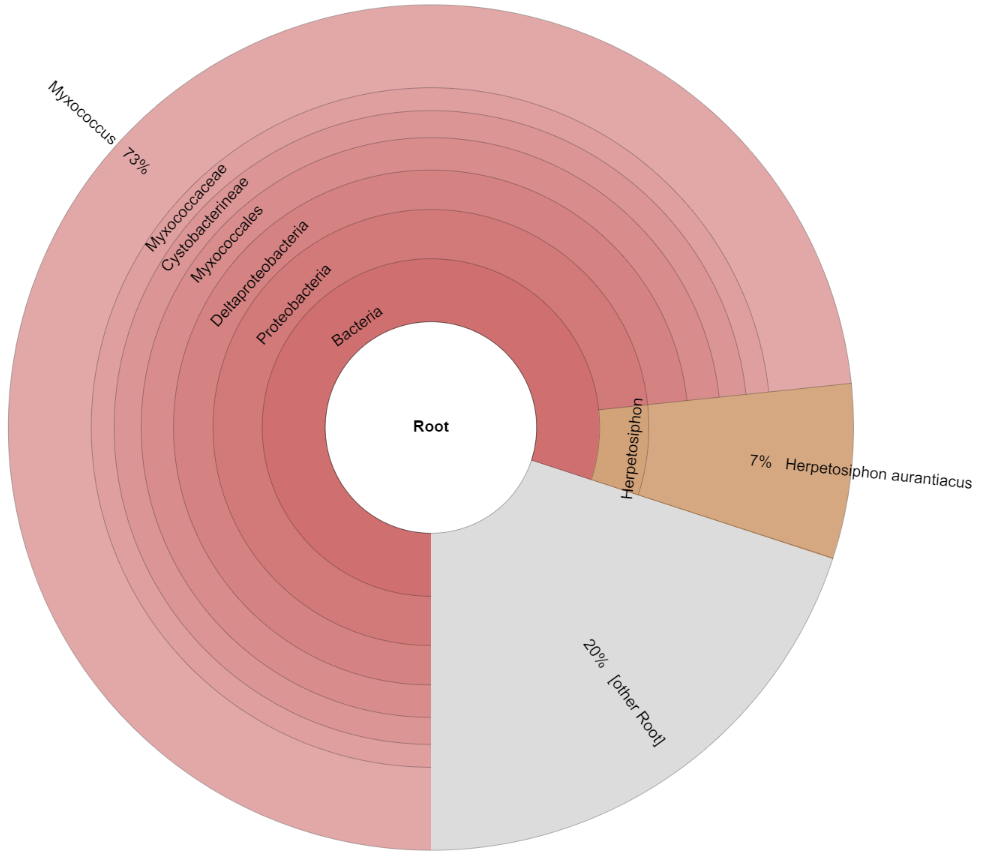
\includegraphics[width=1\textwidth]{figures/results/real/krona/krona-uk-sERR5014633.png}
        \captionof{figure}{Krona for sample ERR5014633}
        \label{fig:results:real:krona-uk-a}
        \end{subfigure}
        \hfill
        \begin{subfigure}[b]{0.52\textwidth}
        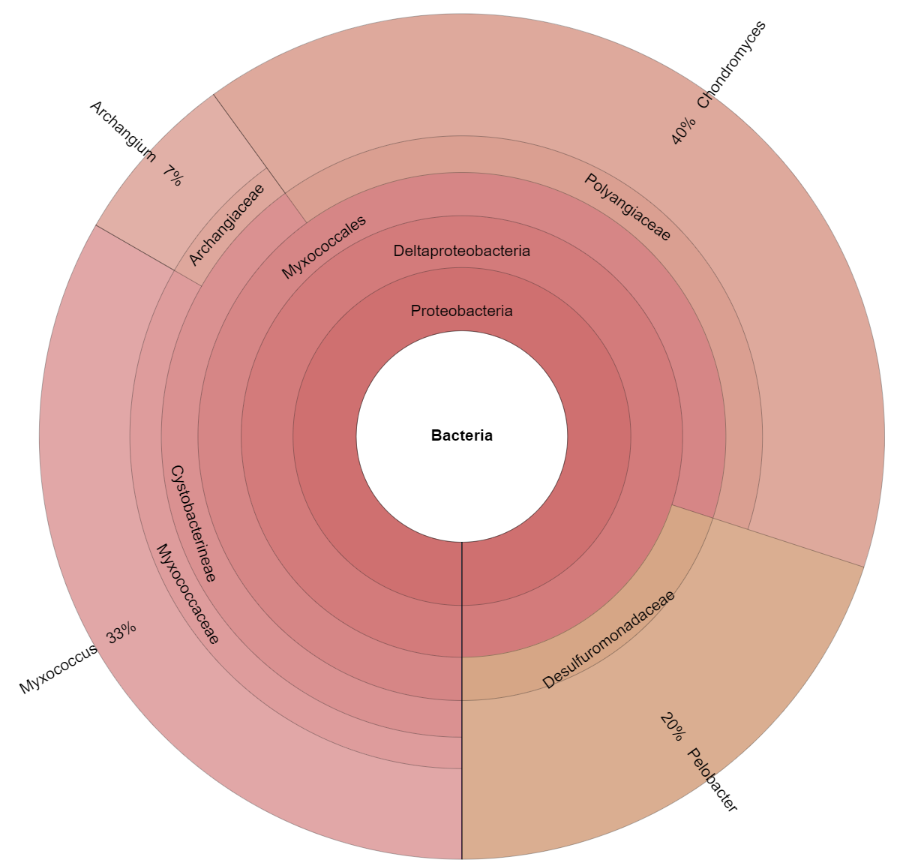
\includegraphics[width=1\textwidth]{figures/results/real/krona/krona-uk-sERR5014683.png}
        \captionof{figure}{Krona for sample ERR5014683}
        \label{fig:results:real:krona-uk-b}
        \end{subfigure}
        \hfill
        \begin{subfigure}[b]{0.45\textwidth}
        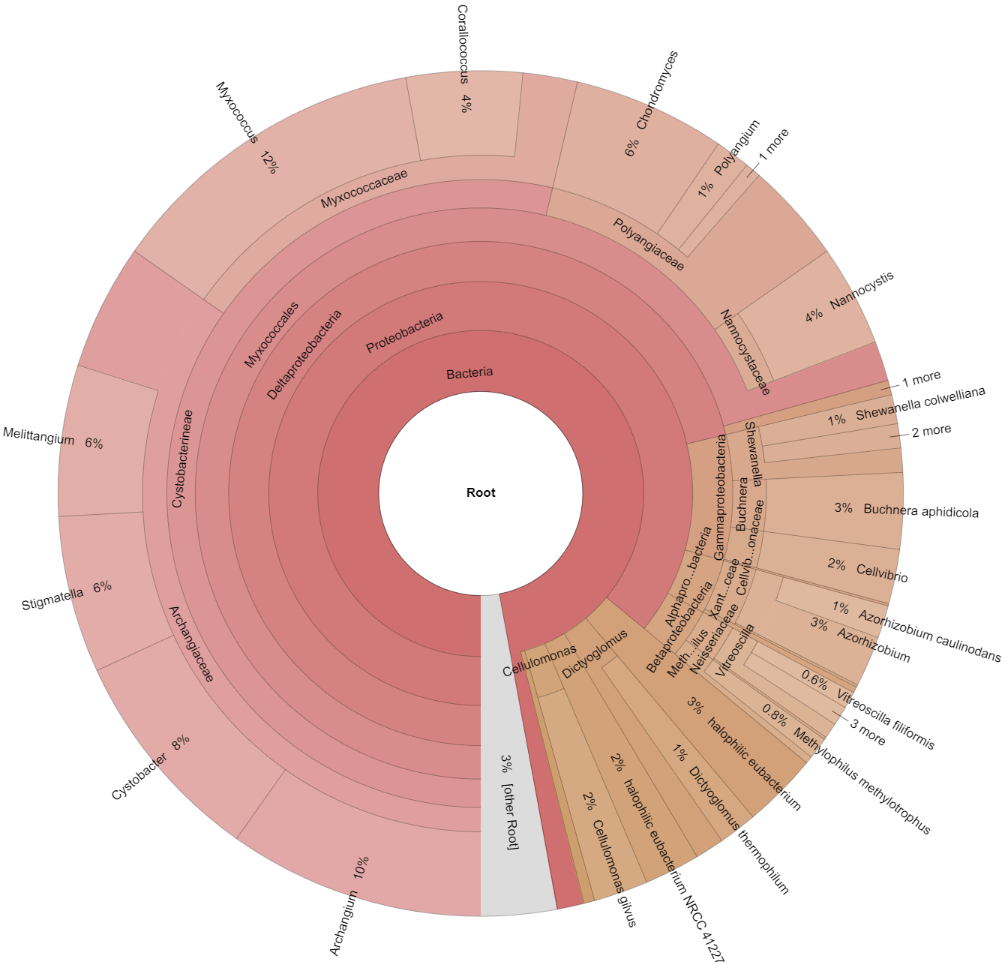
\includegraphics[width=1\textwidth]{figures/results/real/krona/krona-uk-all.png}
        \captionof{figure}{Krona for all aggregated samples}
        \label{fig:results:real:krona-uk-c}
        \end{subfigure}
        \captionof{figure}{Krona chart visualizing the abundances of species in wastewater samples from the UK dataset (PRJEB42191).}
    \end{figure}
    
    The same as to the Californian dataset, for the UK dataset, Freyja labeled all detected variants as “Other”; hence, only non-informative non-interactive plots were generated. Even though Freyja has a limitation while producing an interactive dashboard for too many lineages, for the UK dataset (PRJEB42191), the interactive dashboard was generated (Fig.10). According to the graph, eight lineages were clearly detected by Freyja: i) B.27 that is described in Pango database as “UK lineage, Curacao, Switzerland”; ii) B.23 that was discovered in UK and Portugal; iii) B.12 (Japanese lineage), iv) B.1.14 (USA lineage, California); v) B, one of the two original haplotypes of the pandemic (and first to be discovered); vi) B.1.1.161 (Saudi lineage); vii) B.1.1.514 (US lineage); viii) B.1.1.301 (UK lineage). 
    
    \begin{figure}[ht!]
        \centering
        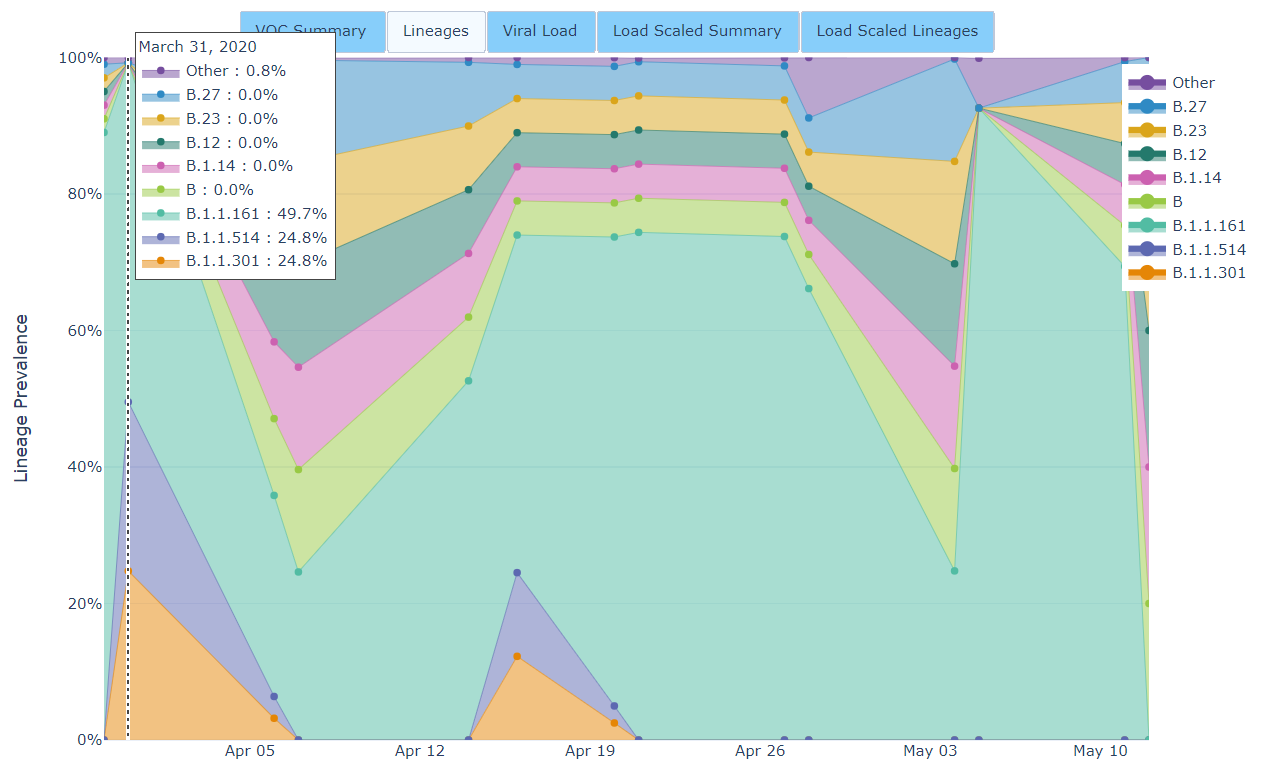
\includegraphics[width=1\textwidth]{figures/results/real/uk-freyja-dash-early-detection.png}
        \captionof{figure}{Interactive dashboard for UK (PRJEB42191) dataset that was generated by Freyja tool as a part of Freyja-based Galaxy workflow.}
        \label{fig:results:real:uk-freyja-dash}
    \end{figure}
    
    Looking at \cref{fig:results:real:uk-freyja-dash}, one can see the prevalence of different lineages over the sample collection time period, from 30 March to 12 May 2020. Detection of B.1.1.514 and B.1.1.301 lineages already at the end of March 2020 (more precisely, in samples collected on 31 March, as well as on 6, 16, and 20 April 2020) is worth mentioning because in Pango database \cite{covlineages} the earliest dates of registration for these lineages is 1 and 22 May 2020, respectively. This fact proves earlier detection within wastewater surveillance over clinical surveillance.





\clearpage
